\documentclass{beamer}

\usepackage[frenchb]{babel}
\usepackage[T1]{fontenc}
\usepackage[utf8]{inputenc}
\usepackage{graphicx}           % insertion d'images

\usetheme{Warsaw}
\setbeamertemplate{headline}{}  % pas de haut de page avec le sommaire intégré


%%%%%%%%%%%%%%%%%
% PRÉAMBULE     %
%%%%%%%%%%%%%%%%%
\title{Hubosans4++}
\subtitle{Soutenance de projet}
\author{}
\date{L2 SPI TP5\\ Janvier 2013}
%%%%%%%%%%%%%%%%%
%%%%%%%%%%%%%%%%%




%%%%%%%%%%%%%%%%%
% BEGIN         %
%%%%%%%%%%%%%%%%%
\begin{document}

    % affichage de la page de titre
    \frame{\titlepage}


    % % % % % % %
    % SOMMAIRE  %
    % % % % % % %
    \begin{frame}
        \tableofcontents[]
    \end{frame}      



    % % % % % % %
    % FRAME 1   %
    % % % % % % %
    \section{Le projet}
    \begin{frame}
    \frametitle{Hubosans4++}
    \framesubtitle{Le puissance 4++}
        Objectif : réaliser un puissance 4 "amélioré", 
            en intégrant notamment les gestions de N joueurs 
            et de trois types de pièces. \\     
        \vspace{2cm} % espace vertical
        Langage : C, compilé par gcc. \\
        %\includegraphics{ressources/presentation/img1.bitmap}
    \end{frame}



    % % % % % % %
    % FRAME 2   %
    % % % % % % %
    \section{Organisation}
    \begin{frame}
    \frametitle{Organisation}
    \framesubtitle{du git, du module et du MVC}
        L'organisation s'est faite autour d'un dépôt git, 
            hébergé par github.  
        \vspace{1cm} % espace vertical
        \begin{columns}[c] % structure en colonne
            \begin{column}{5cm} % colonne de gauche
                Le programme est divisé en modules, en essayant 
                    de respecter au mieux une architecture MVC. 
            \end{column}
            \begin{column}{7cm} % colonne de droite
                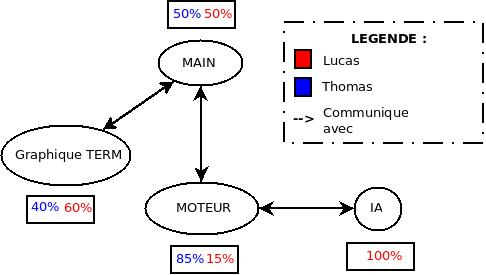
\includegraphics[width=6cm, height=4cm]{ressources/presentation/archi_projet.jpeg}
            \end{column}
        \end{columns}
        \vspace{1cm} % espace vertical
        Autour du programme, plusieurs fichiers d'intérêt.
            (doc, todo list)
    \end{frame}


    % % % % % % %
    % FRAME 3   %
    % % % % % % %
    \section{Les structures de données}
    \begin{frame}
    \frametitle{Les structures de données}
    \framesubtitle{... sont nos amies}
        De nombreuses structures ont été définies, à commencer 
            par les structures de jeu, de joueur, et d'action, 
            les plus importante et utilisées.\\
        \begin{description}
            \item[jeu :] plateau de jeu, liste de joueurs, pile d'actions;\\
            \item[joueur :] id, noms, points, \textit{etc};\\
            \item[action :] enregistre les actions des joueurs. Communication.\\
        \end{description}
    \end{frame}






    % % % % % % %
    % FRAME 4   %
    % % % % % % %
    \section{Méthodes de programmation}
    \begin{frame}
    \frametitle{Méthodes de programmation}
    \framesubtitle{vim, NERD* et bidouillages}
        \begin{columns}[c] % structure en colonne
            \begin{column}{6cm} % colonne de gauche
                \begin{block}{vim}
                    Un standard depuis les temps jadis, puissant et personnalisable.
                \end{block}
            \end{column}
            \begin{column}{5cm} % colonne de droite
                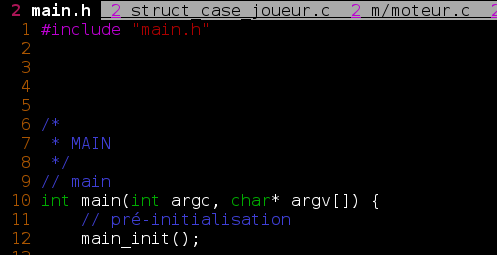
\includegraphics[width=5cm, height=3cm]{ressources/presentation/vim.png}
            \end{column}
        \end{columns}
        \vspace{1cm} % espace vertical
        \begin{exampleblock}{Couplé à des modules d'intérêt}
            fugitive, NERDcommenter, NERDtree, vundle, TeTrIs, taglist... 
        \end{exampleblock}
    \end{frame}




    % % % % % % %
    % FRAME 5   %
    % % % % % % %
    \section{Avantages et limites}
    \begin{frame}
    \frametitle{Avantages et limites}
    \framesubtitle{vers l'infini et au delà}
        \begin{columns}[c] % structure en colonne
            \begin{column}{5.5cm} % colonne de gauche
                \begin{exampleblock}{Avantage}
                    % LISTE
                    \begin{itemize}
                        \item modulable, car modulaire;
                        \item code principal de haut niveau;
                        \item portable;
                    \end{itemize}
                \end{exampleblock}
            \end{column}
            \begin{column}{5.5cm} % colonne de droite
                \begin{alertblock}{Limites}
                    % LISTE
                    \begin{itemize}
                        \item modules trop liés;
                        \item interface grahique pas au top; 
                        \item peu ou pas d'uniformisation générale;
                        \item limites du terminal (nb joueur, simplicité);
                    \end{itemize}
                \end{alertblock}
            \end{column}
        \end{columns}
    \end{frame}




    % % % % % % %
    % FRAME 6   %
    % % % % % % %
    \section{Quelques algorithmes parmi les plus notoires}
    \begin{frame}
    \frametitle{Quelques algorithmes parmi les plus notoires}
    \framesubtitle{Détection de puissance 4}
    	\begin{block}{Calcul-Max}
		    Calcul les valeurs maximales dans toutes les directions pour un points donné. Diminus le nombre de calcul et évite les erreurs de segmentations.\\
	\end{block}
	\begin{block}{Calcul-Pièce}
		    Compte le nombre de pièce à la suite appartenant au même joueur, et ce dans toute les directions. Si ce nombre atteint 4, alors il y a puissance 4.\\
	\end{block}
    \end{frame}




    % % % % % % %
    % FRAME 7   %
    % % % % % % %
    \begin{frame}
    \frametitle{Quelques algorithmes parmi les plus notoires}
    \framesubtitle{Minimax, alpha-bêta}
        \begin{block}{Minimax}
            Parcours de l'arbre des possibilités jusqu'à une certaine profondeur pour trouver la meilleure action possible.
        \end{block}
        \begin{block}{Alpha-Bêta}
            Elagage permettant de ne pas parcourir les branches de l'arbre qui ne sont de toute façon pas plus intéressantes que les autres.\\
            Économie de calcul visible, voir nécessaire.
        \end{block}
    \end{frame}



    % % % % % % %
    % FRAME 8   %
    % % % % % % %
    \section{Bilan}
    \begin{frame}
    \frametitle{Bilan}
    \framesubtitle{return 0;}
        Le projet a été l'occasion :
        \begin{itemize}
            \item d'apprendre à travailler en binôme;
            \item d'apprendre certains aspects de la programmation;
            \item d'échanger des connaissances;
            \item d'apprendre LaTeX;
            \item de concevoir un code de base modulable;
        \end{itemize}

    \end{frame}



%%%%%%%%%%%%%%%%%
% END           %
%%%%%%%%%%%%%%%%%
\end{document}




